\def\baselinestretch{1}
\chapter{Approccio parallelo e implementazione in ambiente GPU} \label{cap:approccio-parallelo}
\chaptermark{Approccio parallelo su GPU}
\def\baselinestretch{1.66}

%%%%%%%%%%%%%%%%%%%%%%%%%%%%%%%%%%%%%%%%%%%%%%%%%%%%%%%%%%%%%%%
%                   Approccio parallelo
%%%%%%%%%%%%%%%%%%%%%%%%%%%%%%%%%%%%%%%%%%%%%%%%%%%%%%%%%%%%%%%
\section{Approccio parallelo} \label{sec:approccio-parallelo}
\noindent Nel capitolo \ref{cap:modello-numerico} sezione \ref{sec:approccio-sequenziale} è stato analizzato l'algoritmo sequenziale per la risoluzione della PDE (Partial Differential Equation) proposta in questo lavoro. A causa dell'elevato tempo di calcolo richiesto dalla procedura sequenziale per trovare la soluzione dell'equazione (\ref{eq:peer-methods-1}) all'aumentare di $N$ (si rimanda alla sezione \ref{sec:sequential_test} per approfondimenti), si è scelto di parallelizzare il modulo relativo al calcolo di tale equazione. Prima di passare direttamente alla presentazione del codice parallelo e della strategia di parallelizzazione adottata, vengono illustrare le operazioni preliminari svolte per la stesura dell'algoritmo parallelo.

%--------------------------------------------------------------
%                   Operazioni preliminari
%--------------------------------------------------------------
\subsection{Operazioni preliminari} \label{subsec:approccio-parallelo-operazioni-preliminari}
\noindent Il primo passo effettuato nel processo di parallelizzazione dell'algoritmo sequenziale \ref{alg:peerMethodsSequential} è stato quello di ottimizzare il modo in cui è memorizzata la matrice $L$ definita in (\ref{eq:matrix-L}). Tale matrice è una matrice tridiagonale a blocchi, che presenta un gran numero di valori nulli che non influiscono in alcun modo nelle operazioni in cui è coinvolta la matrice, rendendo quindi inutile salvarli in memoria. L'approccio che si utilizza in questi casi (e che è stato utilizzato) è quello di memorizzare la matrice $L$ in formato \textit{\textbf{CSR (Compressed Sparse Row)}}. Il formato CSR è pensato per memorizzare una matrice con un gran numero di zeri in maniera compatta, eliminando tutti i valori nulli e memorizzando solo i valori non nulli (chiamati non-zero values, talvolta abbreviato in nnz). Il formato prevede di dichiarare tre array che chiameremo rispettivamente \texttt{row\_ptrs}, \texttt{col\_ids} e \texttt{vals}. L'array \texttt{row\_ptr} fornisce la somma cumulativa degli elementi diversi da zero in ogni riga e quindi ha dimensione $m + 1$ per una matrice sparsa $m \times n$. L'array \texttt{col\_ids} fornisce l'indice della colonna e l'array \texttt{vals} fornisce i valori per ciascuno degli elementi diversi da zero. Pertanto, il formato CSR richiede $2 \times nnz + m + 1$ di spazio di allocazione. Se il numero di nnz è particolarmente ridotto, come nel caso della matrice $L$, si ha una diminuzione sia dello spazio di allocazione e sia nel numero di operazioni che vengono svolte.

\noindent Di seguito si riporta un esempio del formato CSR applicato a una matrice tridiagonale a blocchi $A$ di $4 \times 4$ elementi e con gli indici che partono da 0.

\begin{equation*}
    A = \begin{bmatrix} 
	-2 & 1 & 0 & 1\\
	1 & -2 & 1 & 0\\
	0 & 1 & -2 & 1\\
    1 & 0 & 1 & -2
	\end{bmatrix}
	\quad
\end{equation*}

\begin{equation*}
    \texttt{row\_ptrs} \quad [0 \quad 3 \quad 6 \quad 9 \quad 12] \\
\end{equation*}
\begin{equation*}
    \texttt{col\_idxs} \quad [0 \quad 1 \quad 3 \quad 0 \quad 1 \quad 2 \quad 1 \quad 2 \quad 3 \quad 0 \quad 2 \quad 3] \\
\end{equation*}
\begin{equation*}
    \texttt{vals} \quad [-2 \quad 1 \quad 1 \quad  1 \quad -2 \quad 1 \quad 1 \quad -2 \quad 1 \quad 1 \quad 1 \quad -2] \\
\end{equation*}

%--------------------------------------------------------------
%                   Algoritmo parallelo
%--------------------------------------------------------------
\section{Algoritmo parallelo} \label{subsec:approccio-parallelo-algoritmo-parallelo}
\noindent Lo pseudo-codice parallelo \ref{alg:peerMethodsParallel} evidenzia i passi principali della procedura numerica in un ambiente GPU. I dettagli e le operazioni principali sono elencati nei seguenti passaggi:

\newpage

\begin{breakablealgorithm}
    \caption{Algoritmo parallelo peer methods}\label{alg:peerMethodsParallel}
    \vspace{0.5cm}
    \textbf{Input} $s,x_0,X,N, t_0, T,M, y_0,N, L, a,B_1,B_2,H, F, S, d, D, \Delta t$. \quad
    \textbf{Output} $Y$
    \vspace{0.2cm}
    \begin{algorithmic}[1]
        \Statex \textbf{// Initialization}
        \State $t\_span = [t_0, T]$
        \State time discretization $t_n(n = 0, \ldots, N)$
        \State $N = (t\_span[2]-t\_span[1])/\Delta t$
        \State $x\_span = [x_0, X]$
        \State space discretization $x_m(m = 0, \ldots, M - 1)$
        \State $\Delta x = (x\_span[2]-x\_span[1])/(M - 1)$
        \Statex \textbf{// Sequential spatial discretization}
        \State building of $L_{Diff}$ and $L$ as in \eqref{eq:matrix-Ldiff}, \eqref{eq:matrix-L}
        \State convert $L$ from dense to sparse matrix in CSR format
        \Statex \textbf{// Parallel time discretization using peer method}
        \State $s = 2$
        \Statex // GPU computation start
        \State \texttt{transfer} Input data from Host-To-Device
        \Statex // Initialization with time step $n = 0$
        \State \texttt{parallel computing} of $Y_{0,1}$ and $Y_{0,2}$ using Runge-Kutta 4th order method
        \State \texttt{parallel evaluation} of $\mathcal{F}((Y_{0,1}))$ and $\mathcal{F}((Y_{0,2}))$ as in \eqref{eq:FYnm1-equation}
        \Statex // Main loop: loop on time steps
        \For {$n = 1 \ldots N$} 
        \State \texttt{parallel computing} $Y_{n,1}$ and $Y_{n,2}$ as in \eqref{eq:extended-peer-methods}
        \State \texttt{parallel evaluation} of $\mathcal{F}((Y_{n,1}))$ and $\mathcal{F}((Y_{n,2}))$ as in \eqref{eq:FYnm1-equation}
        \EndFor
        \State \texttt{transfer} Output data from Device-To-Host
        \Statex // GPU computation end
    \end{algorithmic}
\end{breakablealgorithm}
\vspace{0.2cm}
%--------------------------------------------------------------
%                Spiegazione pseudocodice
%--------------------------------------------------------------
\begin{itemize}
    \item \texttt{Righe 2-7}: l'algoritmo inizializza i parametri necessari per la discretizzazione del tempo e dello spazio così come nella controparte sequenziale \ref{alg:peerMethodsSequential}.
    
    \item \texttt{Righe 9-10}: dopo aver definito la matrice $L$ così come è stato fatto nell'algoritmo \ref{alg:peerMethodsSequential}, la si converte in formato CSR (Compressed Sparse Row). L'algoritmo per la definizione della matrice $L$ in formato CSR è il seguente:
    \begin{breakablealgorithm}
        \caption{Definizione matrice in formato CSR}\label{alg:CSRAlg}
        \vspace{0.5cm}
        \textbf{Input} $A, nrows, ncols, nnz$ \\
        \textbf{Output} $row\_ptrs, col\_idxs, values$
        \vspace{0.5cm}
        \begin{algorithmic}[1]
            \State \texttt{allocate} $row\_ptrs[1\ldots nrwos + 1]$
            \State \texttt{allocate} $col\_idxs[1 \ldots nnz]$
            \State \texttt{allocate} $values[1 \ldots nnz]$
            \State $cumulative\_sum = 0$
            \For {$i = 1 \ldots nrows$}
                \State $row\_ptrs[i] = cumulative\_sum$
                \For {$j = 1 \ldots ncols$}
                    \State $col\_idxs[cumulative\_sum] = j$
                    \State $values[cumulative\_sum] = A[i, j]$
                    \State $cumulative\_sum = cumulative\_sum + 1$
                \EndFor
            \EndFor
            \State $row\_ptrs[nrows] = cumulative\_sum$
        \end{algorithmic}
    \end{breakablealgorithm}

    \begin{itemize}
        \item \texttt{Righe 1-4}: inizializzazione e allocazione delle strutture dati ossia $row\_ptrs$, $col\_idxs$, $values$.
        \item \texttt{Righe 5-12}: viene costruita la matrice sparsa. Il ciclo for più esterno costruire l'array $row\_ptrs$, quello più interno $col\_idxs$ e $values$ salvando rispettivamente gli indici di colonna e i valori diversi da zero all'interno di queste due strutture dati.
    \end{itemize}
    
    \item \texttt{Righe 16-17}: si procede con il calcolo di $Y_{0, i}$ dove $i = 1 \ldots s$, utilizzando il metodo Runge-Kutta del quarto ordine, che è stato parallelizzato distribuendo le operazioni di algebra lineare su un opportuno numero di thread. Anche la valutazione della funzione $\mathcal{F}$ è stata parallelizzata, distribuendo le operazioni tra un opportuno numero di thread.
    \newpage
    \begin{breakablealgorithm}
        \caption{Algoritmo di Runge-Kutta parallelo}\label{alg:RK4Alg}
        \vspace{0.5cm}
        \textbf{Input} $h, t_0, y_0$ \\
        \textbf{Output} $y$
        \vspace{0.5cm}
        \begin{algorithmic}[1]
            \Statex // Compute $Y_1$
            \State $Y_1 = y_0$
            \Statex // Compute $Y_2$
            \State \texttt{parallel evaluation} of $\mathcal{F}(Y_1)$
            \State \texttt{parallel product} $h / 2$ by $\mathcal{F}(Y_1)$
            \State $Y_2 =$ \texttt{parallel sum} $y_0 + \mathcal{F}(Y_1)$
            \Statex // Compute $Y_3$
            \State \texttt{parallel evaluation} of $\mathcal{F}(Y_2)$
            \State \texttt{parallel product} $h / 2$ by $\mathcal{F}(Y_2)$
            \State $Y_3 =$ \texttt{parallel sum} $y_0 + \mathcal{F}(Y_2)$
            \Statex // Compute $Y_4$
            \State \texttt{parallel evaluation} of $\mathcal{F}(Y_3)$
            \State \texttt{parallel product} $h$ by $\mathcal{F}(Y_3)$
            \State $Y_4 =$ \texttt{parallel sum} $y_0 + \mathcal{F}(Y_3)$
            \Statex // Make a sort of weighted arithmetic mean
            \State $y = y_0 + h \cdot (1/6 \cdot \mathcal{F}(Y_1) + 1/3 \cdot \mathcal{F}(Y_2) + 1/3 \cdot \mathcal{F}(Y_3) + 1/6 \cdot \mathcal{F}(Y_4))$
        \end{algorithmic}
    \end{breakablealgorithm}
    
    \item \texttt{Righe 20-21}: ancora una volta il loop principale non fa altro che eseguire le stesse operazioni eseguite al di fuori del loop, dato che ogni step è funzione del precedente come è stato ampiamente discusso nel capitolo \ref{cap:modello-numerico}. Si calcola in parallelo $Y_{n, i}$ dove $i = 1 \ldots s$ ed $n = 1 \ldots N$ secondo l'equazione \eqref{eq:peer-methods-1}, eseguendo parallelamente gli $s$ stage della variabile $j$. La valutazione della funzione $\mathcal{F}$ è praticamente la stessa effettuata alla riga \texttt{17}.
\end{itemize}

\noindent Nella paragrafo successivo verrà analizzata in dettaglio la strategia di parallelizzazione utilizzata per il calcolo dell'equazione (\ref{eq:peer-methods-1}) in ambiente CUDA (riga 20 dell'algoritmo parallelo \ref{alg:peerMethodsParallel}), in quanto per la sua importanza merita un approfondimento in più.

%--------------------------------------------------------------
%                   computeYGPU
%--------------------------------------------------------------
\subsection{Strategia di parallelizzazione kernel dell'equazione principale } \label{computeYGPU-par}
\noindent Per capire qual è il processo che ha portato alla parallelizzazione dell'equazione (\ref{eq:peer-methods-1}) in ambiente CUDA, la si può riscrivere in forma più compatta come segue:

\begin{equation}
    Y_{n, i} =  b_{ij}Y_{n - 1, j} + h a_{ij} f(t_{n - 1, j}, Y_{n - 1, j})
    \label{eq:parallel-peer-methods-compressed}
\end{equation}

\begin{equation*}
    \text{con } n = 2\ldots N \quad i = 1\ldots s \quad j = 1\ldots s \nonumber
\end{equation*}

\noindent Poiché $s = 2$, andiamo ad esplicitare la $j$ e otteniamo due equazioni:
\begin{gather}
    Y_{n, 1} =  b_{i1}Y_{n - 1, 1} + h a_{i1} f(t_{n - 1, 1}, Y_{n - 1, 1}) \nonumber \\ 
    Y_{n, 2} =  b_{i2}Y_{n - 1, 2} + h a_{i2} f(t_{n - 1, 2}, Y_{n - 1, 2})
    \label{eq:parallel-peer-methods-unrolled}
\end{gather}

\noindent Una volta ottenuta l'equazione in questa forma, bisogna capire come implementare i vari attori che la compongono. Sia $d$ la dimensione del problema, $Y$ può essere visto come una matrice di dimensione $s \cdot d \times N$, ove i primi $d$ valori rappresentano la soluzione $Y_{n,1}$ e i restanti $d$ valori rappresentano $Y_{n,2}$. $A$ e $B$ sono due matrici $2 \times 2$ la cui configurazione è quella in (\ref{eq:ABc-equation}) e la funzione $f$ viene calcolata seguendo l'equazione \eqref{eq:ODE-system-disc} e poiché la dimensione del problema è $d$, sarà un vettore di $d$ elementi.

\begin{figure}[ht!]
    \centering
    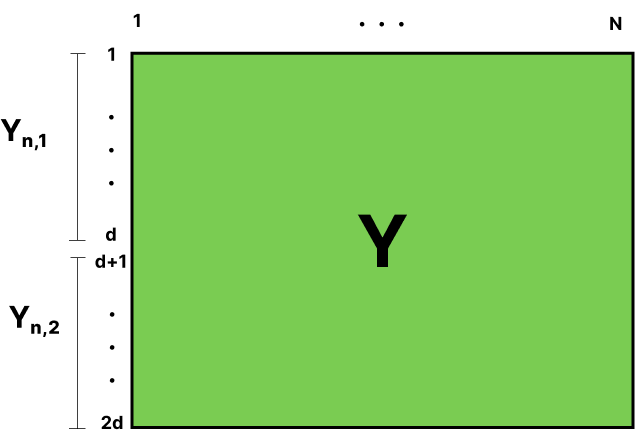
\includegraphics[scale=0.25]{img/MatrixY075x.png}
    \caption{Struttura della matrice Y.}
    \label{fig:matrixYstructure}
\end{figure}

\noindent L'implementazione della strategia di parallelizzazione consiste nel creare un kernel apposito per il calcolo di $Y_{n,1}$ e $Y_{n,2}$ per ogni $n = 2,\ldots,N$ e nello sfruttare l'architettura CUDA, che ci consente di organizzare i thread in blocchi (come spiegato nel capitolo \ref{cap:GPU}). Sia i thread che i blocchi possono essere bidimensionali, cioè è possibile scegliere una griglia di thread all'interno di una griglia di blocchi. I thread presenti nello stesso blocco godono di alcuni vantaggi, come ad esempio possono condividere alcuni registri in modo da eseguire in maniera più efficienti le operazioni assegnate. L'implementazione della strategia di parallelizzazione proposta mira a fare in modo che la griglia con cui viene lanciato il kernel sia bidimensionale, ossia ci siano fissi due blocchi lungo l'asse y e un numero di blocchi lungo l'asse delle x che può essere arbitrario. Anche il numero di thread all'interno di ciascun blocco può essere arbitrario, purché non sia in numero maggiore rispetto agli elementi della matrice $Y$ su cui bisogna operare. La distribuzione del lavoro tra i vari thread e i vari blocchi avviene dividendo la dimensione del problema $d$ per il prodotto tra il numero di thread e il numero di blocchi. Disponendo di una griglia bidimensionale di blocchi, considerando che ciascun blocco ha una coppia di identificativi chiamati rispettivamente \texttt{blockIdx.x} e \texttt{blockIdx.y}, i blocchi con \texttt{blockIdx.y} = 0 calcoleranno l'equazione (\ref{eq:parallel-peer-methods-unrolled}) per $i = 1$ e i blocchi con \texttt{blockIdx.y} = 1 calcoleranno la medesima equazione per $i = 2$ concorrentemente. Osservando la figura \ref{fig:matrixYstructure} si può notare che ciascun stage $i$ opera su porzioni differenti della matrice $Y$ e questo fa sì che non possano verificarsi race condition sugli elementi della matrice.

\begin{figure}[ht!]
    \centering
    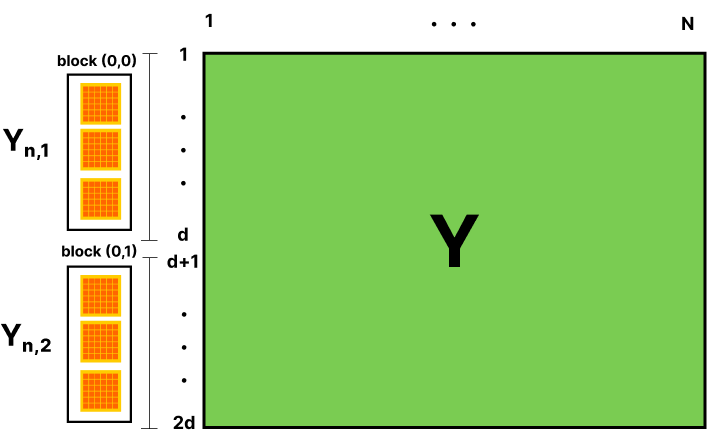
\includegraphics[scale=0.35]{img/YwBlocks.png}
    \caption{Distribuzione dei valori della matrice $Y$ fra thread e blocchi.}
    \label{fig:matrixYstructure}
\end{figure}